% !TeX root = ../main.tex
\chapter{Przygotowanie}
\label{chap:cooking}

\section{Kroki}
\label{sec:steps}

\begin{enumerate}
  \item Mięso zalać zimną wodą i powoli doprowadzić do wrzenia.
  \item Zebrać szumowiny łyżką cedzakową.
  \item Dodać warzywa i przyprawy, zmniejszyć ogień do minimum.
  \item Gotować tak, żeby zupa ledwo \enquote{mrugała} -- około \num{8} \ac{bpm}.
\end{enumerate}

Ustawienie garnka na kuchence pokazano na rysunku~\ref{fig:pot}.

% The caption goes BELOW a figure. Real figures go in figures/ (PDF from
% draw.io, PNG for screenshots); this one is drawn with TikZ.
\begin{figure}[htbp]
  \centering
  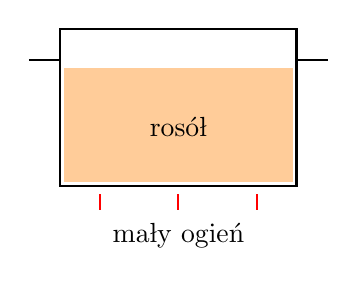
\begin{tikzpicture}
    \draw[thick] (0,0) rectangle (3,2);
    \draw[thick] (-0.4,1.6) -- (0,1.6);
    \draw[thick] (3,1.6) -- (3.4,1.6);
    \fill[orange!40] (0.05,0.05) rectangle (2.95,1.5);
    \node at (1.5,0.75) {rosół};
    \foreach \x in {0.5,1.5,2.5} \draw[red, thick] (\x,-0.3) -- (\x,-0.1);
    \node[below] at (1.5,-0.35) {mały ogień};
  \end{tikzpicture}
  \caption{Garnek z rosołem na małym ogniu}
  \label{fig:pot}
\end{figure}

\section{Czas gotowania}
\label{sec:time}

Czas gotowania $t$ (w godzinach) zależy od masy mięsa $m$ (w kilogramach) i wyraża się wzorem
\begin{equation}
  t = 1{,}5 + 0{,}6 \cdot m ,
  \label{eq:time}
\end{equation}
co dla porcji z tabeli~\ref{tab:ingredients} daje $t = \num{2.4}$~h.
\supervisor{Skąd ten wzór? Brak źródła!}

\section{Automatyzacja}
\label{sec:automation}

Przeliczanie składników na inną liczbę porcji wykonuje funkcja \code{scale_recipe} z listingu~\ref{lst:scale}.
Kod wczytywany jest wprost z pliku, więc w dokumencie jest zawsze jego aktualna wersja.

\lstinputlisting[
  language=Python,
  caption={Przeliczanie składników (plik \texttt{scripts/scale\_recipe.py})},
  label={lst:scale},
]{scripts/scale_recipe.py}
